\documentclass{beamer}
%
% Choose how your presentation looks.
%
% For more themes, color themes and font themes, see:
% http://deic.uab.es/~iblanes/beamer_gallery/index_by_theme.html
%
\mode<presentation>
{
  \usetheme{default}      % or try Darmstadt, Madrid, Warsaw, ...
  \usecolortheme{default} % or try albatross, beaver, crane, ...
  \usefonttheme{default}  % or try serif, structurebold, ...
  \setbeamertemplate{navigation symbols}{}
  \setbeamertemplate{caption}[numbered]
} 

\addtobeamertemplate{navigation symbols}{}{%
    \usebeamerfont{footline}%
    \usebeamercolor[fg]{footline}%
    \hspace{1em}%
    \insertframenumber/\inserttotalframenumber
}

\usepackage[english]{babel}
\usepackage[utf8x]{inputenc}

\title[Završni rad]{Klasifikacija uporabom umjetnih
neuronskih mreža}

\author{Darijo Brčina}
\institute{Sveučilište u Zagrebu \linebreak \textbf{Fakultet elektrotehnike i računarstva} \linebreak \linebreak Završni rad br. 6950}
\date{Zagreb, 06.07.2020}

\begin{document}

\begin{frame}
  \titlepage
\end{frame}

% Uncomment these lines for an automatically generated outline.
\begin{frame}{Sadržaj}
  \tableofcontents
\end{frame}

\section{Opis zadatka}
	\begin{frame}{Opis zadatka}
		Cilj:
		\begin{itemize}
			\item naučiti neuronsku mrežu da na temelju danih labeliranih podataka jasno može odrediti kojem razredu pripadaju
		\end{itemize}

		\bigskip
		\bigskip
		
		\begin{figure}
			\pause
			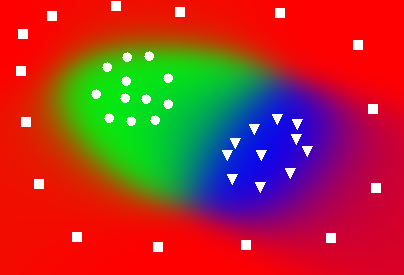
\includegraphics[scale=0.5]{img/cilj_slika.png}
		\end{figure}
	\end{frame}

\section{Nadzirano učenje}
	\begin{frame}{Nadzirano učenje}
		\begin{itemize}
			\pause
			\item Jedno od glavnih područja strojnog učenja
			\pause
			\item Model nadziranog učenja (engl. \textit{supervised learning}) prolazi kroz dvije faze:
			\bigskip
			\begin{figure}
			    \pause
			    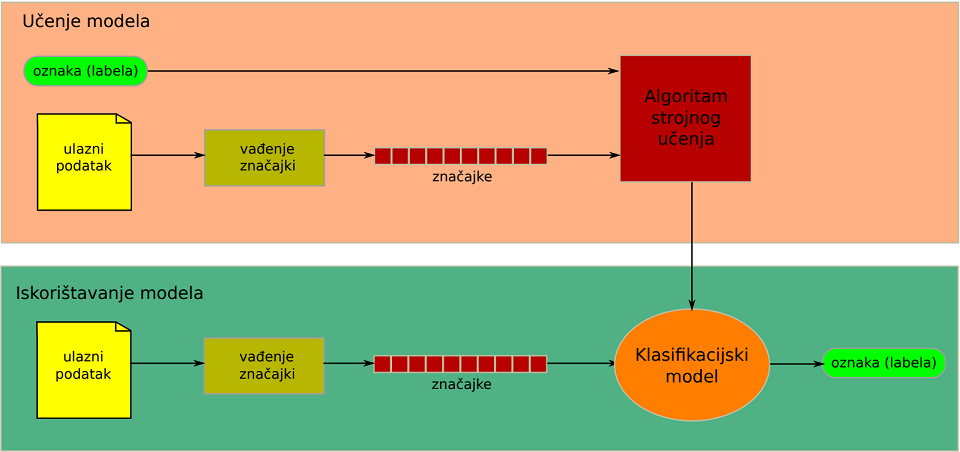
\includegraphics[scale=0.35]{img/supervised-learning-flow.png}
		    \end{figure}
		    \bigskip
		    \pause
		    \item Glavni cilj je omogućiti da model razvije svojstvo \textbf{generalizacije}
		    \pause
		    \item Ispostavlja se da je to dosta zahtjevno za izvesti pa često dolazi do problema \textbf{prenaučenosti} (engl. \textit{overfitting})
		\end{itemize}
	\end{frame}
	\begin{frame}{Lijek za prenaučenost}
	    \begin{itemize}
	        \pause
	        \item Prenaučenost je jedan od glavnih problema strojnog učenja koji model čini beskorisnim zbog loše generalizacije
	        \pause
	        \item Jedan od načina kako spriječiti prenaučenost je korištenje metode \textbf{unakrsna provjera} (engl. \textit{cross-validation})
	        \pause
	        \item Ideja je da se oko 30\% uzoraka \textbf{skupa za učenje} (engl. \textit{training set}) prebaci u \textbf{skup za provjeru} (engl. \textit{validation set}) te prati pogreška nad oba skupa pomoću koje ćemo odrediti kada je učenje modela potrebno zaustaviti:
	        \smallskip
	        \pause
	        \begin{figure}
			    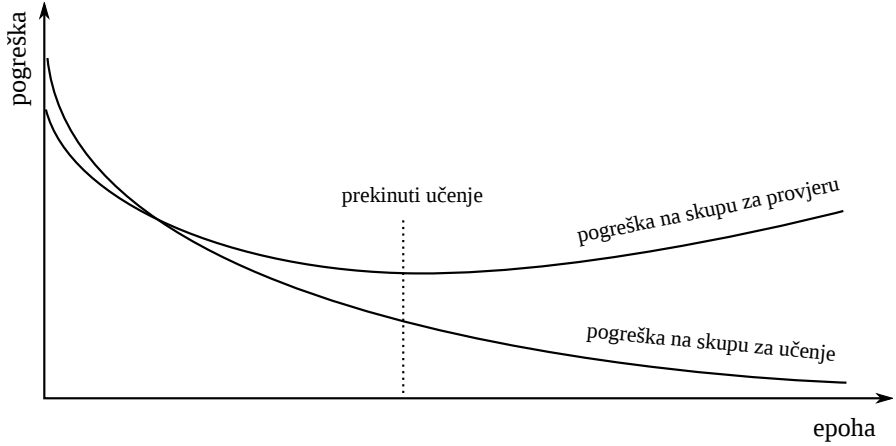
\includegraphics[scale=0.35]{img/cross-validation.png}
		    \end{figure}
	    \end{itemize}
	\end{frame}
    \begin{frame}{Skup za testiranje}
        \begin{itemize}
            \pause
            \item Ponekad su modeli složeni pa je potrebno odrediti njihovu optimalnu složenost te se zbog toga uvodi \textbf{skup za testiranje} (engl. \textit{testing set}) koji također sadrži oko 30\% uzoraka skupa za učenje i služi za provjeru točnosti jednom naučenog modela
            \pause
            \item Slikovito prikazani skupovi:
            \bigskip
            \begin{figure}
			    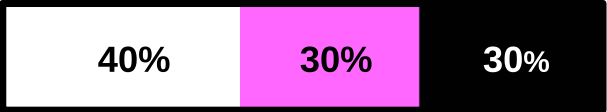
\includegraphics[scale=0.35]{img/skupovi.png}
		    \end{figure}
        \end{itemize}
    \end{frame}

\subsection{Problemi nadziranog učenja}
    \subsubsection{Regresija}
        \begin{frame}{Problemi nadziranog učenja - Regresija}
            \begin{itemize}
                \pause
                \item Regresija (engl. \textit{regression}) je tehnika kojom se pokušava modelirati odnos između određenog broja značajki i kontinuirane ciljne varijable
                \pause
                \item Razlikujemo više tipova regresija poput linearne i nelinearne 
                regresije kao i regresije s jednom varijablom i regresije s više varijabli
                \pause
                \begin{figure}
                    \begin{subfigure}
                        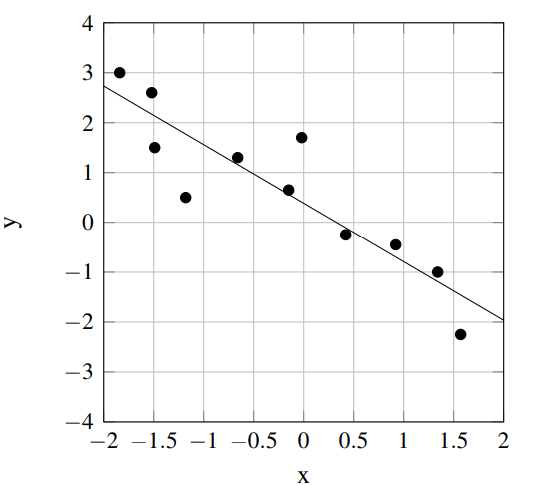
\includegraphics[scale=0.3]{img/linear-regression.png}
                    \end{subfigure}
                    \begin{subfigure}
                        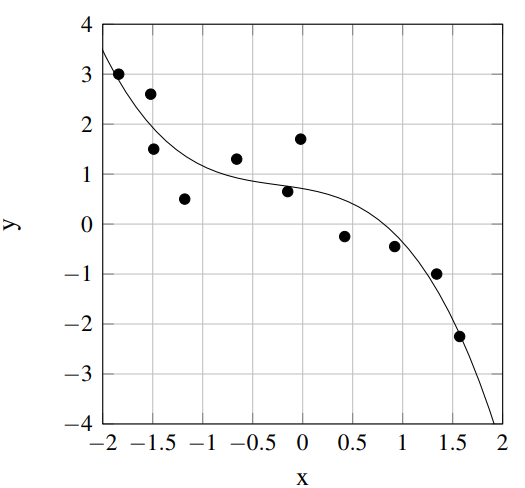
\includegraphics[scale=0.3]{img/polynom-regression.png}
                    \end{subfigure}
                \end{figure}
            \end{itemize}
        \end{frame}
    \subsubsection{Klasifikacija}
        \begin{frame}{Problemi nadziranog učenja - Klasifikacija}
            \begin{itemize}
                \pause
                \item Klasifikacija (engl. \textit{classification}) je tehnika kojom se određene oznake pokušavaju kategorizirati diskretnim vrijednostima
                \pause
                \item Kao i kod regresije, razlikujemo linearnu i nelinearnu klasifikaciju
                \pause
                \item Razlikujemo binarnu i višerazrednu klasifikaciju i klasifikaciju više oznaka
                \bigskip
                 \pause
                \begin{figure}
                    \begin{subfigure}
                        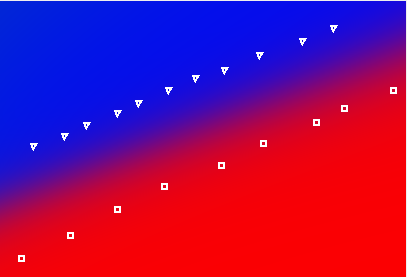
\includegraphics[scale=0.35]{img/linear-classification.png}
                    \end{subfigure}
                    \begin{subfigure}
                        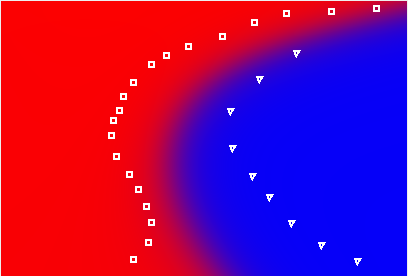
\includegraphics[scale=0.35]{img/non-linear-classification.png}
                    \end{subfigure}
                \end{figure}
            \end{itemize}
        \end{frame}

\section{Umjetne neuronske mreže}
    \begin{frame}{Umjetne neuronske mreže}
        \begin{itemize}
            \pause
            \item Jedan od najkorištenijih algoritama strojnog učenja
            \pause
            \item Motivacija pronađena u građi, povezanosti i brzini obrade raznih podražaja ljudskog mozga te mogućnosti učenja iz prijašnjeg iskustva
            \pause
            \item Danas je poznato da u ljudskom mozgu postoji oko 10\textsuperscript{11} neurona te 10\textsuperscript{15} međusobnih veza, što znači da je svaki neuron u prosjeku povezan s 10\textsuperscript{4} različitih veza
            \pause
            \item Primjer konektivističkog pristupa
            \pause
            \item Područje koje se bavi proučavanjem umjetnih neuronskih mreža naziva se neuro računarstvo (engl. \textit{neuro-computing}) koje je jedno od grana mekog računarstva (engl. \textit{soft-computing}) 
        \end{itemize}
    \end{frame}
    \begin{frame}{Umjetne neuronske mreže}
        \begin{figure}
            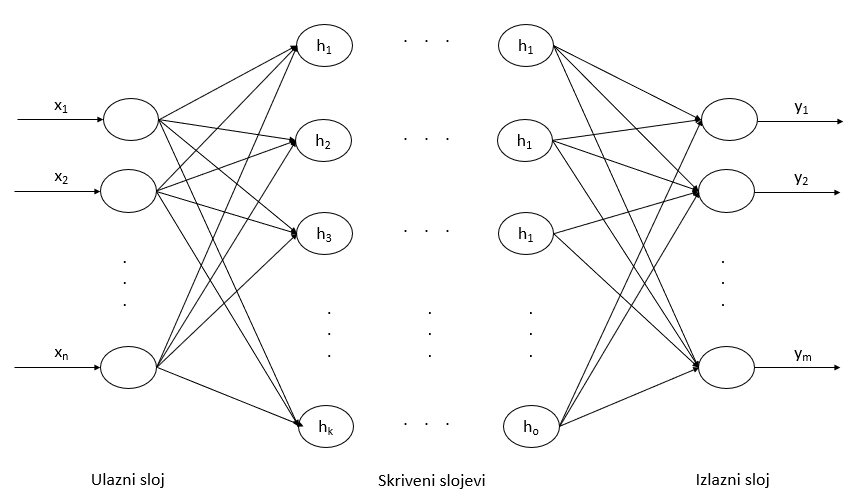
\includegraphics[scale=0.3]{img/ann.png}
        \end{figure}
        \begin{figure}
            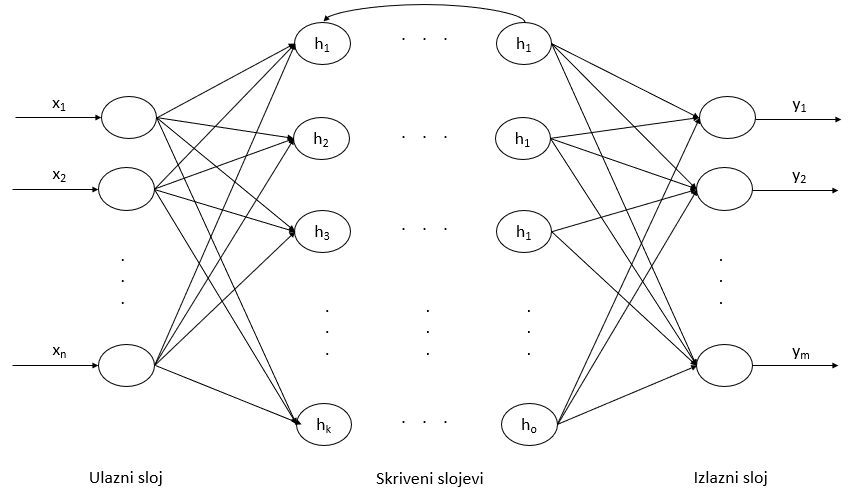
\includegraphics[scale=0.3]{img/cycle-ann.png}
        \end{figure}
    \end{frame}
    
    \subsection{Umjetni neuron}
        \begin{frame}{Umjetni neuron}
            \begin{itemize}
                \pause
                \item Motiviran strukturom biološkog neurona:
                \begin{figure}
                    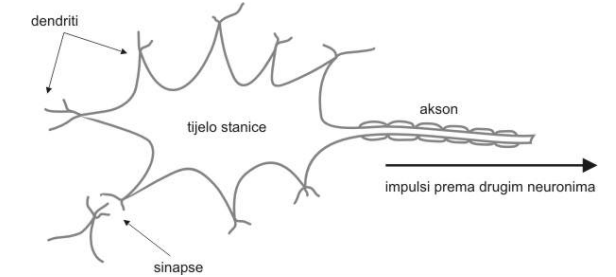
\includegraphics[scale=0.5]{img/bio-neuron.png}
                \end{figure}
                \pause 
                \item Definiran 1943.\ u radu \textit{A Logical Calculus of Ideas Immanent in Nervous Activity} dvojice znastvenika Warren S. McCulloch i Walter H. Pitts
            \end{itemize}
        \end{frame}
        \begin{frame}{Umjetni neuron}
           \begin{itemize}
                \begin{figure}
                    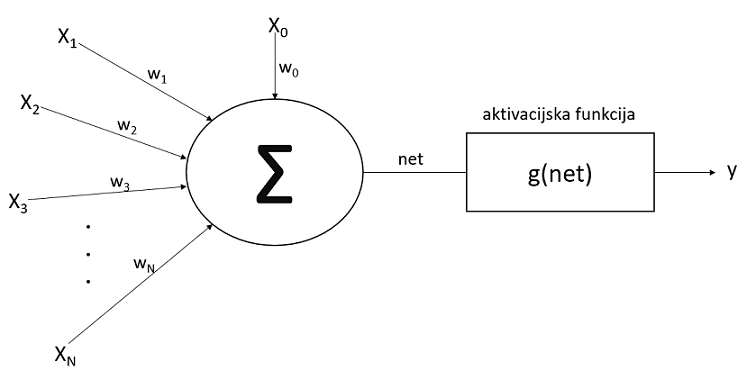
\includegraphics[scale=0.36]{img/ai-neuron.png}
                \end{figure}
                \pause
                \item Sastoji se od $(n+1)$ različitih ulaza \textbf{x} i težina \textbf{w} te jednog izlaza \textbf{y}
                \pause
                \item Izlaz se dobije tako što se prvo izračuna \textbf{net} vrijednost po formuli: \[net = \sum\limit_{i=0}^Nx\textsubscript{i} \cdot w\textsubscript{i}\]
                \pause
                \item Zatim se dobivena \textbf{net} vrijednost provuče kroz neku od aktivacijskih funkcija
            \end{itemize}
        \end{frame}
        
    \subsection{Aktivacijske funkcije}
        \begin{frame}{Aktivacijske funkcije}
            
        \end{frame}
    
    \subsection{Unaprijedna neuronska mreža}
        \begin{frame}{Unaprijedna neuronska mreža}
            
        \end{frame}
    
    \subsection{Učenje unaprijedne neuronske mreže}
        \begin{frame}{Učenje unaprijedne neuronske mreže}
            
        \end{frame}

\section{Rezultati}	
	\begin{frame}{Rezultati}
		
	\end{frame}


\section{Zaključak}
	\begin{frame}{Zaključak}
		\begin{itemize}
			\item Segmentacija uvelike ovisi o kvaliteti pretprocesiranja
			\smallskip
			\item Vrlo je teško postići izrazito visoku točnost
		\end{itemize}
		
		\bigskip		
		\pause		
		
		\begin{block}{Mogući nastavci na ovaj rad}
			\begin{itemize}
				\item Dalje poboljšavati postupak segmentacije postojećeg pristupa
				\item Isprobati nesegmentacijski pristup rješavanju ovog problema
			\end{itemize}
		\end{block}
	\end{frame}

\end{document}